% Options for packages loaded elsewhere
\PassOptionsToPackage{unicode}{hyperref}
\PassOptionsToPackage{hyphens}{url}
\PassOptionsToPackage{dvipsnames,svgnames,x11names}{xcolor}
%
\documentclass[
  letterpaper,
  DIV=11,
  numbers=noendperiod]{scrartcl}

\usepackage{amsmath,amssymb}
\usepackage{iftex}
\ifPDFTeX
  \usepackage[T1]{fontenc}
  \usepackage[utf8]{inputenc}
  \usepackage{textcomp} % provide euro and other symbols
\else % if luatex or xetex
  \usepackage{unicode-math}
  \defaultfontfeatures{Scale=MatchLowercase}
  \defaultfontfeatures[\rmfamily]{Ligatures=TeX,Scale=1}
\fi
\usepackage{lmodern}
\ifPDFTeX\else  
    % xetex/luatex font selection
\fi
% Use upquote if available, for straight quotes in verbatim environments
\IfFileExists{upquote.sty}{\usepackage{upquote}}{}
\IfFileExists{microtype.sty}{% use microtype if available
  \usepackage[]{microtype}
  \UseMicrotypeSet[protrusion]{basicmath} % disable protrusion for tt fonts
}{}
\makeatletter
\@ifundefined{KOMAClassName}{% if non-KOMA class
  \IfFileExists{parskip.sty}{%
    \usepackage{parskip}
  }{% else
    \setlength{\parindent}{0pt}
    \setlength{\parskip}{6pt plus 2pt minus 1pt}}
}{% if KOMA class
  \KOMAoptions{parskip=half}}
\makeatother
\usepackage{xcolor}
\setlength{\emergencystretch}{3em} % prevent overfull lines
\setcounter{secnumdepth}{5}
% Make \paragraph and \subparagraph free-standing
\makeatletter
\ifx\paragraph\undefined\else
  \let\oldparagraph\paragraph
  \renewcommand{\paragraph}{
    \@ifstar
      \xxxParagraphStar
      \xxxParagraphNoStar
  }
  \newcommand{\xxxParagraphStar}[1]{\oldparagraph*{#1}\mbox{}}
  \newcommand{\xxxParagraphNoStar}[1]{\oldparagraph{#1}\mbox{}}
\fi
\ifx\subparagraph\undefined\else
  \let\oldsubparagraph\subparagraph
  \renewcommand{\subparagraph}{
    \@ifstar
      \xxxSubParagraphStar
      \xxxSubParagraphNoStar
  }
  \newcommand{\xxxSubParagraphStar}[1]{\oldsubparagraph*{#1}\mbox{}}
  \newcommand{\xxxSubParagraphNoStar}[1]{\oldsubparagraph{#1}\mbox{}}
\fi
\makeatother


\providecommand{\tightlist}{%
  \setlength{\itemsep}{0pt}\setlength{\parskip}{0pt}}\usepackage{longtable,booktabs,array}
\usepackage{calc} % for calculating minipage widths
% Correct order of tables after \paragraph or \subparagraph
\usepackage{etoolbox}
\makeatletter
\patchcmd\longtable{\par}{\if@noskipsec\mbox{}\fi\par}{}{}
\makeatother
% Allow footnotes in longtable head/foot
\IfFileExists{footnotehyper.sty}{\usepackage{footnotehyper}}{\usepackage{footnote}}
\makesavenoteenv{longtable}
\usepackage{graphicx}
\makeatletter
\newsavebox\pandoc@box
\newcommand*\pandocbounded[1]{% scales image to fit in text height/width
  \sbox\pandoc@box{#1}%
  \Gscale@div\@tempa{\textheight}{\dimexpr\ht\pandoc@box+\dp\pandoc@box\relax}%
  \Gscale@div\@tempb{\linewidth}{\wd\pandoc@box}%
  \ifdim\@tempb\p@<\@tempa\p@\let\@tempa\@tempb\fi% select the smaller of both
  \ifdim\@tempa\p@<\p@\scalebox{\@tempa}{\usebox\pandoc@box}%
  \else\usebox{\pandoc@box}%
  \fi%
}
% Set default figure placement to htbp
\def\fps@figure{htbp}
\makeatother
% definitions for citeproc citations
\NewDocumentCommand\citeproctext{}{}
\NewDocumentCommand\citeproc{mm}{%
  \begingroup\def\citeproctext{#2}\cite{#1}\endgroup}
\makeatletter
 % allow citations to break across lines
 \let\@cite@ofmt\@firstofone
 % avoid brackets around text for \cite:
 \def\@biblabel#1{}
 \def\@cite#1#2{{#1\if@tempswa , #2\fi}}
\makeatother
\newlength{\cslhangindent}
\setlength{\cslhangindent}{1.5em}
\newlength{\csllabelwidth}
\setlength{\csllabelwidth}{3em}
\newenvironment{CSLReferences}[2] % #1 hanging-indent, #2 entry-spacing
 {\begin{list}{}{%
  \setlength{\itemindent}{0pt}
  \setlength{\leftmargin}{0pt}
  \setlength{\parsep}{0pt}
  % turn on hanging indent if param 1 is 1
  \ifodd #1
   \setlength{\leftmargin}{\cslhangindent}
   \setlength{\itemindent}{-1\cslhangindent}
  \fi
  % set entry spacing
  \setlength{\itemsep}{#2\baselineskip}}}
 {\end{list}}
\usepackage{calc}
\newcommand{\CSLBlock}[1]{\hfill\break\parbox[t]{\linewidth}{\strut\ignorespaces#1\strut}}
\newcommand{\CSLLeftMargin}[1]{\parbox[t]{\csllabelwidth}{\strut#1\strut}}
\newcommand{\CSLRightInline}[1]{\parbox[t]{\linewidth - \csllabelwidth}{\strut#1\strut}}
\newcommand{\CSLIndent}[1]{\hspace{\cslhangindent}#1}

\KOMAoption{captions}{tableheading}
\makeatletter
\@ifpackageloaded{caption}{}{\usepackage{caption}}
\AtBeginDocument{%
\ifdefined\contentsname
  \renewcommand*\contentsname{Table of contents}
\else
  \newcommand\contentsname{Table of contents}
\fi
\ifdefined\listfigurename
  \renewcommand*\listfigurename{List of Figures}
\else
  \newcommand\listfigurename{List of Figures}
\fi
\ifdefined\listtablename
  \renewcommand*\listtablename{List of Tables}
\else
  \newcommand\listtablename{List of Tables}
\fi
\ifdefined\figurename
  \renewcommand*\figurename{Figure}
\else
  \newcommand\figurename{Figure}
\fi
\ifdefined\tablename
  \renewcommand*\tablename{Table}
\else
  \newcommand\tablename{Table}
\fi
}
\@ifpackageloaded{float}{}{\usepackage{float}}
\floatstyle{ruled}
\@ifundefined{c@chapter}{\newfloat{codelisting}{h}{lop}}{\newfloat{codelisting}{h}{lop}[chapter]}
\floatname{codelisting}{Listing}
\newcommand*\listoflistings{\listof{codelisting}{List of Listings}}
\makeatother
\makeatletter
\makeatother
\makeatletter
\@ifpackageloaded{caption}{}{\usepackage{caption}}
\@ifpackageloaded{subcaption}{}{\usepackage{subcaption}}
\makeatother

\usepackage{bookmark}

\IfFileExists{xurl.sty}{\usepackage{xurl}}{} % add URL line breaks if available
\urlstyle{same} % disable monospaced font for URLs
\hypersetup{
  pdftitle={Linking Education, Unemployment, and Poverty},
  pdfauthor={Isis Martinez},
  colorlinks=true,
  linkcolor={blue},
  filecolor={Maroon},
  citecolor={Blue},
  urlcolor={Blue},
  pdfcreator={LaTeX via pandoc}}


\title{Linking Education, Unemployment, and Poverty\thanks{Project
repository available at:
\url{https://github.com/iterrall/MATH261A-project-1-martinez}.}}
\usepackage{etoolbox}
\makeatletter
\providecommand{\subtitle}[1]{% add subtitle to \maketitle
  \apptocmd{\@title}{\par {\large #1 \par}}{}{}
}
\makeatother
\subtitle{Insights from California's CalEnviroScreen Data}
\author{Isis Martinez}
\date{September 25, 2025}

\begin{document}
\maketitle
\begin{abstract}
We analyze the relationship between educational attainment and poverty
in California with CalEnviroScreen 4.0, which is a statewide screening
tool developed by the Office of Environmental Health Hazard Assessment
(OEHHA). With a simple linear regression of census-tract location
poverty rates on the percentage of adults without a high school diploma,
we show that each one-point increase in low educational attainment is
associated with an increase in poverty rate. This model shows about
61.6\% of California tract-level variation in poverty, and is only
minimally impacted when accounting for unemployment. This report will
also share diagnostics of the model that indicate a lack of residual
normality and variance constancy, so we interpret interval estimates
with caution. These findings highlight the value of CalEnviroScreen for
identifying socioeconomic vulnerability and informing policies aimed at
reducing poverty and inequality.
\end{abstract}


\section{Introduction}\label{sec-intro}

The link between educational attainment to socioeconomic well-being has
been widely corroborated in research (for example, Cutler and
Lleras-Muney (2006) and Zajacova and Lawrence (2018)). The persistent
geographic inequities California faces drives the need for us to take a
closer look at how education relates to poverty when related to
location. Therefore, using the CalEnviroScreen 4.0 dataset, (Office of
Environmental Health Hazard Assessment (OEHHA) 2021), we ask the
following question in this project: \textbf{To what extent is
tract-level poverty associated with low levels of education in
California?}.

Understanding this question can be an important way to learn poverty
disparity mitigation techniques within communities to improve health,
since low socioeconomic status has been tied to multiple environmental
risks and health disparities Morello-Frosch and Shenassa (2006).

We address this question by fitting a simple linear regression by taking
poverty rate as a function of percentage of adults lacking a high school
diploma. We then extend the analysis by exploring the contribution of
unemployment makes on the model and examining the robustness of linear
regression model assumptions.

The remainder of this paper is structured as follows:
Section~\ref{sec-data} discusses the data, Section~\ref{sec-methods} the
model and the methods we used, Section~\ref{sec-results} presents the
results, and Section~\ref{sec-discussion} discusses the conclusions in
addition to weaknesses with the conclusions from this model.

\section{Data}\label{sec-data}

In 2021, The California Environmental Protection Agency published its
most recent version of the California Communities Environmental Health
Screening tool, which is also known as CalEnviroScreen 4.0 (California
Office of Environmental Health Hazard Assessment (OEHHA) 2021a). Since
its original release in 2013, CalEnviroScreen has compiled and analyzed
census-tract data in California. While its primary focus is to better
understand and address environmental concerns in California communities,
we can learn a great deal from the raw data that can be found on the
CalEnviroScreen Data Hub (Office of Environmental Health Hazard
Assessment (OEHHA) 2021) about possible socioeconomic well-being
predictors and outcomes. There is a wealth of information around
geospatial data that can be used to drive more equitable decision-making
by exploring possible factors that play a role in changes to poverty
levels.

We use the data from CalEnviroScreen 4.0 that uses data from the US
Census Bureau's American Community Survey (ACS) that collects
information on educational attainment annually (California Office of
Environmental Health Hazard Assessment (OEHHA) 2021b).

This dataset provides socioeconomic, health, and environmental measures,
and our observational units are census tracts in California. For this
analysis, we focus on the 2019 values of socioeconomic indicators from
the Office of Environmental Health Hazard Assessment (OEHHA) (2021):

\begin{itemize}
\item
  \textbf{Poverty (pov)}: Percent of the population living below two
  times the federal poverty level (5-year estimate, 2015-2019) within
  each California census tract. Multiplying the federal poverty level is
  to account for the high cost of living in California.
\item
  \textbf{Education (edu)}: Percent of adults that are 25+ years old
  without a high school diploma. This percentage was derived as 100
  minus the share of adults with high school or higher education levels
  (estimated over 5 years, 2015-2019)
\item
  \textbf{Unemployment (unemp)}: Percent of the labor force that is
  unemployed.
\end{itemize}

The data on educational attainment and poverty come 5-year estimates
from 2015--2019 that come from the American Community Survey (ACS) (U.S.
Census Bureau (2014); U.S. Census Bureau (n.d.)) and were presented
within the Office of Environmental Health Hazard Assessment (OEHHA)
(2021) dataset. We follow OEHHA's indicator methods (California Office
of Environmental Health Hazard Assessment (OEHHA) (2021b)), and we note
that ACS estimates include margins of error. OEHHA uses standard error
and corresponding SE screening to flag unreliable tracts. We remove
tracts with missing values in our analysis, with a total of 7906 for our
primary model and 7658 for our model including unemployment as a
variable. All variables are percentages in between 0 and 100,
facilitating coefficient interpretation as percentage-point changes.
which facilitates our coefficient interpretation as changes in
percentage-point.

Our interpretation of regression coefficients are represented as
marginal changes in poverty rate per one-percentage-point change in
education or unemployment. Possible limitations include rounding of
reported percentages, geographic clustering effects not captured by the
model, and the bounded nature of the data (0--100\%), which can produce
heteroskedastic residuals in linear regression.

\begin{longtable}[]{@{}lrrrrrrrr@{}}

\caption{\label{tbl-summ}Descriptive summaries for key variables (tract
level).}

\tabularnewline

\toprule\noalign{}
variable & mean & sd & min & p25 & median & p75 & max & n \\
\midrule\noalign{}
\endhead
\bottomrule\noalign{}
\endlastfoot
pov & 31.33 & 18.21 & 1 & 16.3 & 27.8 & 44.3 & 93.2 & 7658 \\
edu & 17.56 & 14.65 & 0 & 5.8 & 12.7 & 26.1 & 76.3 & 7658 \\
unemp & 6.26 & 3.77 & 0 & 3.6 & 5.5 & 8.0 & 41.1 & 7658 \\

\end{longtable}

Descriptive summaries show that poverty rates, education, and
unemployment are all highly variable across tracts as shown in the table
Table~\ref{tbl-summ} that reports key summaries from our data. A
scatterplot of poverty versus education (Figure~\ref{fig-pov-scatter})
suggests a positive linear trend, while unemployment also shows a
positive but weaker association with poverty
(Figure~\ref{fig-pov-other}).

\section{Methods}\label{sec-methods}

To investigate the relationship between poverty rates and educational
attainment, we adopt a simple linear regression model with poverty as
the response and low-educational rate as the predictor. Let \(Y_i\)
denote the percentage of the population living under the poverty
threshold in census tract \(i\), and let \(X_i\) denote the percentage
of adults without a high-school diploma in the same tract.

\[Y_i = \beta_0 + \beta_1X_i + \varepsilon_i \text{ for }i=1,...,n\]

where \(\beta_0\) (the intercept) represents the expected poverty rate
in a census tract when \(X_i=0\), or when 0\% of the adult population is
living without a high school diploma. Additionally, \(\beta_1\)
represents the marginal change in poverty (percentage points) for one
point increase in \(X_i\), or adults without a high school diploma.
Finally, \(\varepsilon_i\) denotes a random error term that encapsulates
unobserved factors that impact poverty rates not explained by
low-educational attainment percentage. In other words, we estimate a
simple linear regression pov =\(\beta_0 + \beta_1\)(edu) +
\(\varepsilon\) using OLS in R (R Core Team 2024; Gelman, Hill, and
Vehtari 2021; Kutner et al. 2005).

The parameters of the model (\(\beta_0\) and \(\beta_1\)) are estimated
using ordinary least squares, or OLS. We estimate parameters with
ordinary least squares (OLS) with R (version 4.5.1) (R Core Team 2024;
Kutner et al. 2005) using the built-in lm() function, which fits linear
regression models by OLS. The basic syntax is lm(response
\textasciitilde{} predictor, data = dataset), and in our case the
function lm(pov \textasciitilde{} edu, data = to\_analyze\_df). This
instructs R to regress the poverty rate (pov) on the percentage of
adults without a high school diploma (edu) using the dataset that we
have turned into a cleaned dataframe that omits null values. Here, pov
is the response variable (dependent variable),edu is the predictor
variable (independent variable), and the \textasciitilde{} operator
indicates the model formula, meaning ``pov'' is modeled as a function of
``edu''. The function estimates the intercept \(\beta_0\) and slope
\(\beta_1\) by minimizing the sum of squared residuals. By default, lm()
returns a model object that contains the estimated coefficients,
residuals, fitted values, and summary statistics, which we accessed
using functions such as summary() and coef().

To assess model fit, we report the estimated regression coefficients,
standard errors, and coefficient of determination (\(R^2\)), and the
associated confidence interval with our the correlation. We also present
a scatterplot (Figure~\ref{fig-pov-scatter})of the data with the fitted
regression line and a confidence band, which provides a visual
assessment of model fit. As a robustness check, we fit a supplemental
multiple linear regression including unemployment:

\[Y_i = \beta_0 + \beta_1X_i + \beta_2U_i +\varepsilon_i \text{ for }i=1,...,n\]

where \(U_i\) represents the unemployment percentage, and \(\beta_2\) is
the slope on unemployment. This would be the expected change in the
poverty rate for 1 percentage-point increase in unemployment, if
education level is constant.

For this OLS, we adopt the standard assumptions of the linear regression
model:

\textbf{1. Linearity}: The relationship between educational attainment
and poverty is linear.

\textbf{2. Independence of errors}: The error terms \(\varepsilon_i\)
are independent between different census tracts.

\textbf{3. Constant variance}: the error terms have constant variance
across values of \(X_i\) (the low-educational attainment rate for census
tract \(i\)). \textbf{4. Normality of residuals}: the residuals are
approximately normally distributed, meaning the error terms have a mean
of zero and are normally distributed.

Because rates are bounded between 0 and 100, having a constant variance
is unlikely. Therefore, we complete the following diagnostics and note
implications for inference to evaluate whether the model comply with the
assumptions of linear regression:

\begin{itemize}
\item
  \textbf{Residual plot}: We examine a scatterplot of residuals versus
  fitted values (Figure~\ref{fig-pov-scatter}) to assess linearity,
  independence of errors, and constant variance (Wickham 2016). A random
  scatter of residuals would indicate that the linearity and constant
  variance assumptions are reasonable.
\item
  \textbf{Normality of residuals}: We use a Q--Q plot
  (Figure~\ref{fig-pov-qq}) using R Core Team (2024) and a histogram of
  residuals (Figure~\ref{fig-pov-histo}) using Wickham (2016) to check
  whether they approximately follow a normal distribution. Additionally,
  we inspected other factors on poverty rates that were contained in the
  dataset such as unemployment (Figure~\ref{fig-pov-other}) (Wickham
  2016). Overall, the diagnostics provide evidence about the level of
  estimated coefficient reliability and inference validity from the
  model. Any violations of assumptions are noted and discussed in
  Section~\ref{sec-results} and Section~\ref{sec-discussion}.
\end{itemize}

We conducted all analyses R (R Core Team 2024), and regression models
were estimated using the base R function \texttt{lm()}. The model
summaries and tidy coefficient tables were generated with the
\texttt{broom} package (Robinson 2014). We used dplyr (Wickham 2016)
(part of the tidyverse) to clean the raw data, and we formatted tables
with (\textbf{Xie2015.We?}) produced visualizations with
\texttt{ggplot2} (Wickham 2016), with additional support from
\texttt{scales} Wickham and Seidel (2022) for scaling and Nascimento
(2019) for Q--Q plotting. Together, these packages helped us create data
cleaning, regression modeling, and visualization that can be
reproducible.

\section{Results}\label{sec-results}

The simple linear regression of poverty level on education yields the
following fitted model:

\(\widehat{pov}=\) 14.255 \(+\) 0.979 \(\times(edu)\) with \(R^2=\)
0.616 and number of tracts = 7906.

In our data (number of tracts = 7906), the estimated intercept is
\(\hat{\beta_0}\)= 14.255 and estimated slope is
\(\hat{\beta_1}\)=0.979. In a supplementary model including
unemployment, the fitted slope for education is with number of tracts
equaling 7658 , the estimated intercept is \(\hat{\beta_0}=\) 7.91 and
estimated slope is \(\hat{\beta_1}=\) 0.838 with \(R^2\) = 0.688.

\textbf{Here is our interpretation of the coefficients}:

\begin{itemize}
\item
  The intercept \(\beta_0 \approx\) 14.255, so for a tract with 100\% of
  its adults holding at least a high school diploma (or 0\% lacking
  one), this model would predict the poverty rate to be an average of
  14.26\% in that tract.
\item
  The slope \(\beta_1 \approx\) 0.979. In other words, each one-percent
  increase in adults without a high-school diploma per census tract
  corresponds to an average 0.98\% increase in poverty rate in that
  tract.
\item
  The model fit \(R^2=\) 0.62, so about 61.59\% of the variation in the
  poverty rate we are measuring is explained by low-education attainment
  percentage within a census-tract.
\item
  The rounded \(p\)-value for education is \textless2e-16
  (\(p < 0.001\)), which is far below common thresholds. This indicates
  that the observed data is not more extreme than the rejection region
  and the association is statistically significant (meaning this is very
  unlikely due to chance). Therefore, both coefficients are noteworthy.
\end{itemize}

\begin{figure}

\centering{

\pandocbounded{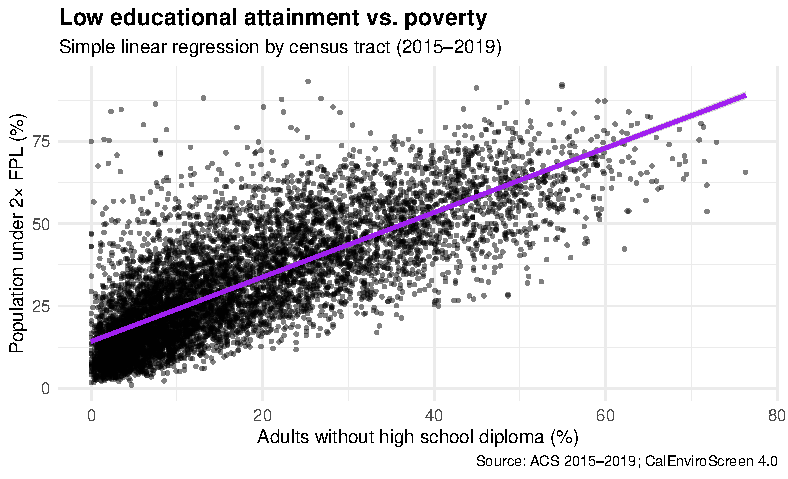
\includegraphics[keepaspectratio]{math261a_martinez_paper_files/figure-pdf/fig-pov-scatter-1.pdf}}

}

\caption{\label{fig-pov-scatter}Scatter plot of percentage of adults
without a high school diploma by California census-tract (x-axis) and
percentage of population in same tract living under two times the
Federal poverty line (FPL) (y-axis) with fitted linear regression
model.}

\end{figure}%

We added a \textbf{supplemental model} with unemployment included to
measure if another factor changes our results significantly. The
education effect remains positive (0.838), and overall fit improves
minimally (\(R^2 =\) 0.688, number of tracts 7658). When unemployment
was added to the regression, the coefficient for education remained
remarkable, but unemployment showed a weaker association with poverty.
The overall model fit improved only slightly with the increase in
\(R^2\). This suggests that differences in unemployment rates across
tracts do not account for most of the variation in poverty once
educational attainment is considered.

\begin{figure}

\centering{

\pandocbounded{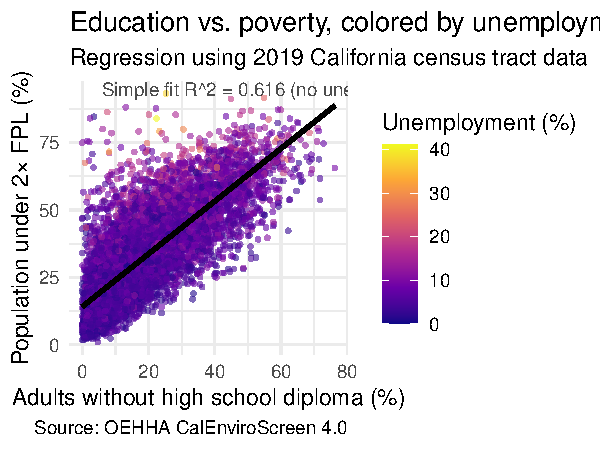
\includegraphics[keepaspectratio]{math261a_martinez_paper_files/figure-pdf/fig-pov-other-1.pdf}}

}

\caption{\label{fig-pov-other}Education vs.~poverty with points colored
by unemployment. The black line shows the simple OLS fit of poverty on
education only; color reveals that higher-unemployment tracts tend to
lie higher in the scatter, but the fitted line does not adjust for
unemployment.}

\end{figure}%

From our model, we find a 95\% confidence interval for the education
slope is approximately equal to {[}0.96166, 0.99574{]}. This means we
are 95\% confident that for each additional percentage point increase in
adults without a high school diploma, the poverty rate of the same
census tract will increase between 0.96166 and 0.99574 percentage
points.

Below, we use visualize the diagnostics to help with our assessment of
the validity of our confidence interval for our primary simple
regression:

\begin{figure}

\centering{

\pandocbounded{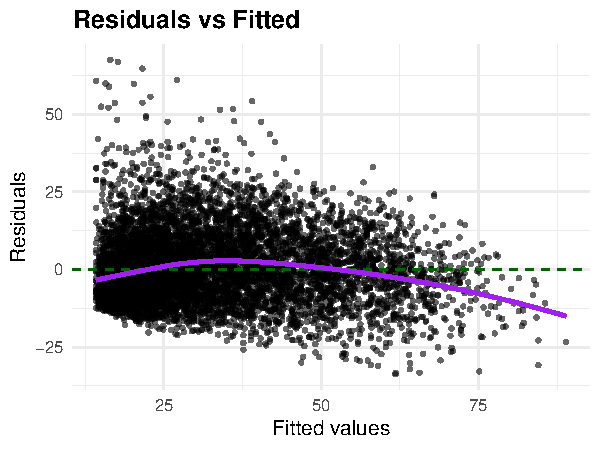
\includegraphics[keepaspectratio]{math261a_martinez_paper_files/figure-pdf/fig-pov-resids-1.pdf}}

}

\caption{\label{fig-pov-resids}Scatter plot of fitted values (x-axis)
and residuals (y-axis) for a simple linear regression with poverty
(percentage of population in census-tract living under two times the
Federal poverty line - FPL) as the response and education (percentage of
adults without a high school diploma) in same tract by the predictor.}

\end{figure}%

\begin{figure}

\centering{

\pandocbounded{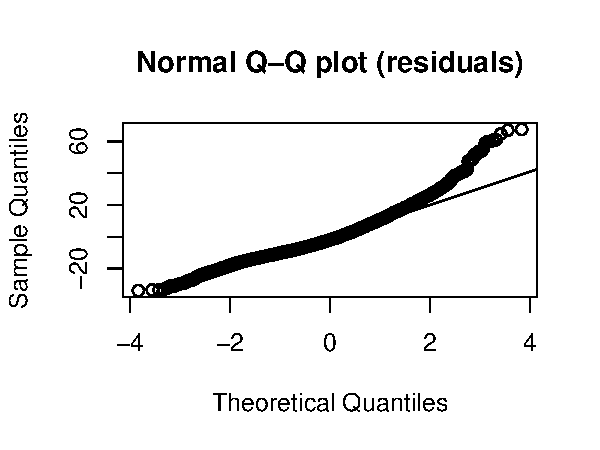
\includegraphics[keepaspectratio]{math261a_martinez_paper_files/figure-pdf/fig-pov-qq-1.pdf}}

}

\caption{\label{fig-pov-qq}Normal Q--Q plot for the primary model's
residuals with poverty as the poverty percentage as response and
education as the predictor. If residuals were normally distributed, the
points would closely follow the reference line. Any curvature and
deviations in the tails suggest that the residuals are not perfectly
normal, with evidence of skewness and heavy tails.}

\end{figure}%

\begin{figure}

\centering{

\pandocbounded{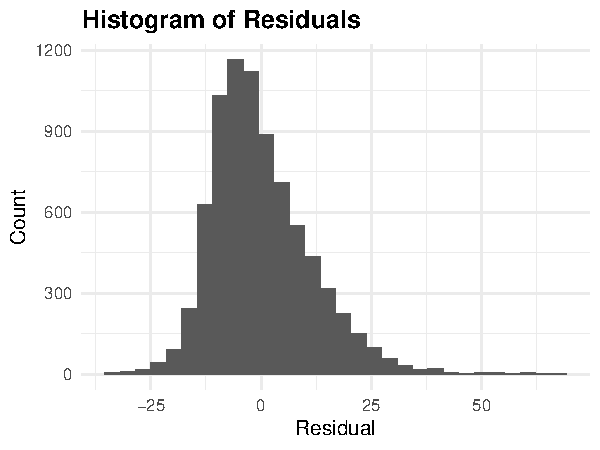
\includegraphics[keepaspectratio]{math261a_martinez_paper_files/figure-pdf/fig-pov-histo-1.pdf}}

}

\caption{\label{fig-pov-histo}Histogram of regression residuals. A
normal distribution of errors would appear bell-shaped and symmetric
around zero. Any residuals that display skewness and heavy tails,
indicate that the normality assumption is not fully satisfied.}

\end{figure}%

Additionally, we conduct a hypothesis test to formally evaluate whether
education is associated with poverty. Let our type I error rate be
\(\alpha = 0.05\). Let us test the following hypotheses:

\(H_0\): \(\beta_1 = 0\) (no relationship between education and poverty)
vs.~\(H_a\): \(\beta_1 \neq 0\).

The t-test for the education coefficient yields a large test statistic
(\(t \approx 113\)) with a p-value less than 0.001. Because the p-value
\(<\alpha=0.05\), we reject \(H_0\) and conclude that low educational
attainment is associated with higher poverty rates at the census tract
level. As an additional note, when unemployment is included in the
supplemental model, the education effect remains relevant, while the
unemployment coefficient is comparatively weaker. This suggests that
unemployment alone does not explain most of the variation in poverty
once education is accounted for.

\section{Discussion}\label{sec-discussion}

\textbf{Summary}: The slope is positive and statistically significant,
so we can conclude that the poverty rate tends to be higher in locations
where there is a higher percentage of adults with lower levels of
education than high school diplomas. If the linear regression
assumptions are true, the results we see in Section~\ref{sec-results}
indicate a moderate effect size in the data that suggest low-education
attainment is a relevant predictor when predicting poverty rate
(although not the only factor) .

\textbf{Model assumptions}: Our diagnostic plots show us several
violations of the classical linear regression assumptions. Linearity
appears reasonable from the Figure~\ref{fig-pov-scatter}, but
independence of errors is unlikely given clustering in
Figure~\ref{fig-pov-resids}, and the residuals show variability and
non-normality in Figure~\ref{fig-pov-resids} and
Figure~\ref{fig-pov-qq}. If the residuals were approximately normal, the
black dots would fall close to the straight diagonal line of the Q-Q
plot. With thousands of tracts, coefficient estimates are stable, but
standard errors may be understated under OLS assumptions. However, the
plot bends upwards both in the lower and upper tails. These issues limit
the precision of our inference and confidence interval. Additionally,
the histogram of residuals (Figure~\ref{fig-pov-histo}) appears
approximately bell-shaped and centered near zero, which supports the
assumption that the errors have mean zero. However, the distribution is
not perfectly symmetric: the right tail is longer than the left, and
there are some extreme positive residuals. This indicates mild right
skew and the presence of high-poverty tracts where the model
underpredicts. While the residuals do not follow a perfect normal
distribution, the large sample size (n = 7906) reduces concerns about
inference validity due to the Central Limit Theorem. Nevertheless, the
skewness suggests that robust standard errors or a variance-stabilizing
transformation (e.g., square-root of the response) might provide more
reliable inference in future analyses. Overall though, the non-normality
and changes in variance, our 95\% confidence interval should only be
drawn cautiously, so we might want to consider using more robust
standard errors.

\textbf{Comparing education and unemployment}: When we added
unemployment to the model, it did not meaningfully change the estimated
effect of education. The unemployment has a weaker positive association
with poverty, but the education coefficient remains consequential. This
result challenges a possible assumption that unemployment is a primary
driver of poverty. We see from Figure~\ref{fig-pov-other} that a high
percentage of individuals are employed but remain below twice the
federal poverty threshold California Office of Environmental Health
Hazard Assessment (OEHHA) (2021b) set. This indicates situations where
many individuals are working but still fall below the poverty threshold
here. By comparison, educational attainment shows a stronger and more
consistent relationship with poverty, which highlights its relevance as
a key factor of socioeconomic well-being.

Generally speaking, the simple linear regression analysis for this
research question can only draw questionable inferences, so the linear
regression is likely not a full picture of the relationship between
education and poverty. With that being said, we did see that the
positive correlation in the linear regression model is likely
statistically significant due to the p-value and \(R^2\) value.
Therefore, there is a positive relationship between low education
attainment percentage and poverty rate percentage.

\textbf{Implications}: We see that the findings support noting education
as a factor in determining predictors of poverty in datasets like
CalEnviroScreen, which are used to identify communities experiencing
socioeconomic and environmental burdens. Policymakers and advocates can
use this data to inform investments in education, workforce support, and
pollution reduction to advance environmental justice and public health.

\textbf{Limitations}: We used cross-sectional, observational data, which
limits our causal inferences. The nature of tract-level geographical
dependence of the data likely violates the independence assumption.
Additionally, the bounded percentage outcomes produce
heteroskedasticity. Finally the ACS sampling error introduces
measurement error.

On a broader level, a limitation of our analysis is the definition of
poverty. CalEnviroScreen uses 200\% of the federal poverty level (FPL)
to account for California's high cost of living. This is a more
appropriate benchmark than the unadjusted FPL, it does not capture wide
regional differences within the state. For example, housing costs in the
Bay Area vs rural areas of California have a large range. Consequently,
the same income threshold may reflect very different levels of economic
hardship depending on location. This limitation means that our poverty
measure may overstate poverty in some rural areas and understate it in
high-cost metropolitan regions, which could feasibly introduce
additional variation not explained by education or unemployment in our
models. Another limitation is that the education measure applies only to
adults aged 25 and older, but the poverty measure covers the entire
population. This mismatch means that our predictor and outcome are not
measured on exactly the same group. For example, tracts with many
children in poverty but relatively well-educated adults could weaken the
observed association. On the other side, tracts with low adult education
may experience higher poverty rates even among children and elderly
residents who are not part of the education measure. This difference in
denominators introduces another possible measurement error into our
regression.

\section{References}\label{references}

\phantomsection\label{refs}
\begin{CSLReferences}{1}{0}
\bibitem[\citeproctext]{ref-OEHHA_MapsData}
California Office of Environmental Health Hazard Assessment (OEHHA).
2021a. {``CalEnviroScreen 4.0: Maps \& Data.''} California Environmental
Protection Agency. \url{https://oehha.ca.gov/calenviroscreen/maps-data}.

\bibitem[\citeproctext]{ref-OEHHA2021}
---------. 2021b. {``CalEnviroScreen 4.0: Updated Analysis.''}
California Environmental Protection Agency.
\url{https://oehha.ca.gov/sites/default/files/media/downloads/calenviroscreen/report/calenviroscreen40reportf2021.pdf}.

\bibitem[\citeproctext]{ref-cutler2006education}
Cutler, David M., and Adriana Lleras-Muney. 2006. {``Education and
Health: Evaluating Theories and Evidence.''} \emph{NBER Working Paper
Series}, no. 12352. \url{https://www.nber.org/papers/w12352}.

\bibitem[\citeproctext]{ref-gelman_regression_2021}
Gelman, Andrew, Jennifer Hill, and Aki Vehtari. 2021. \emph{Regression
and {Other} {Stories}}. Cambridge University Press.

\bibitem[\citeproctext]{ref-kutner2005}
Kutner, Michael H., Christopher J. Nachtsheim, John Neter, and William
Li. 2005. \emph{Applied Linear Statistical Models}. 5th ed. New York:
McGraw-Hill/Irwin.

\bibitem[\citeproctext]{ref-morello2006environmental}
Morello-Frosch, Rachel, and Edmond D. Shenassa. 2006. {``Environmental
Justice and the Distribution of Pollution: The Case of California's
Central Valley.''} \emph{Environmental Health Perspectives} 114 (12):
1810--17. \url{https://doi.org/10.1289/ehp.9310}.

\bibitem[\citeproctext]{ref-qqplotr}
Nascimento, Luis Augusto Perdigão do. 2019. \emph{Qqplotr:
Quantile-Quantile Plots for Ggplot2}.
\url{https://CRAN.R-project.org/package=qqplotr}.

\bibitem[\citeproctext]{ref-oehha_calenviroscreen_dataset}
Office of Environmental Health Hazard Assessment (OEHHA). 2021.
{``CalEnviroScreen Data Hub.''}
\url{https://calenviroscreen-oehha.hub.arcgis.com/\#Data}.

\bibitem[\citeproctext]{ref-R2024}
R Core Team. 2024. \emph{R: A Language and Environment for Statistical
Computing}. Vienna, Austria: R Foundation for Statistical Computing.
\url{https://www.R-project.org/}.

\bibitem[\citeproctext]{ref-robinson2014broom}
Robinson, David. 2014. {``Broom: An r Package for Converting Statistical
Analysis Objects into Tidy Data Frames.''} \emph{arXiv Preprint
arXiv:1412.3565}. \url{https://arxiv.org/abs/1412.3565}.

\bibitem[\citeproctext]{ref-census_portal}
U.S. Census Bureau. n.d. {``Data.census.gov.''}
\url{https://data.census.gov/cedsci/}.

\bibitem[\citeproctext]{ref-acs_tech}
---------. 2014. {``American Community Survey Design and Methodology
Report.''}
\url{https://www2.census.gov/programs-surveys/acs/methodology/design_and_methodology/acs_design_methodology_ch12_2014.pdf}.

\bibitem[\citeproctext]{ref-Wickham2016}
Wickham, Hadley. 2016. \emph{Ggplot2: Elegant Graphics for Data
Analysis}. New York: Springer.

\bibitem[\citeproctext]{ref-scales}
Wickham, Hadley, and Dana Seidel. 2022. \emph{Scales: Scale Functions
for Visualization}. \url{https://CRAN.R-project.org/package=scales}.

\bibitem[\citeproctext]{ref-zajacova2018}
Zajacova, Anna, and Elizabeth M. Lawrence. 2018. {``Education and
Health: The Casual Association and Challenges.''} \emph{Annual Review of
Public Health} 39: 273--89.
\url{https://doi.org/10.1146/annurev-publhealth-031816-044628}.

\end{CSLReferences}




\end{document}
